% Appendix A


%----------------------------------------------------------------------------------------
%----------------------------------------------------------------------------------------
%----------------------------------------------------------------------------------------
\chapter{Detailed high-level description of the components of \textit{RootSkel}}


\begin{table}[H]
	\centering
	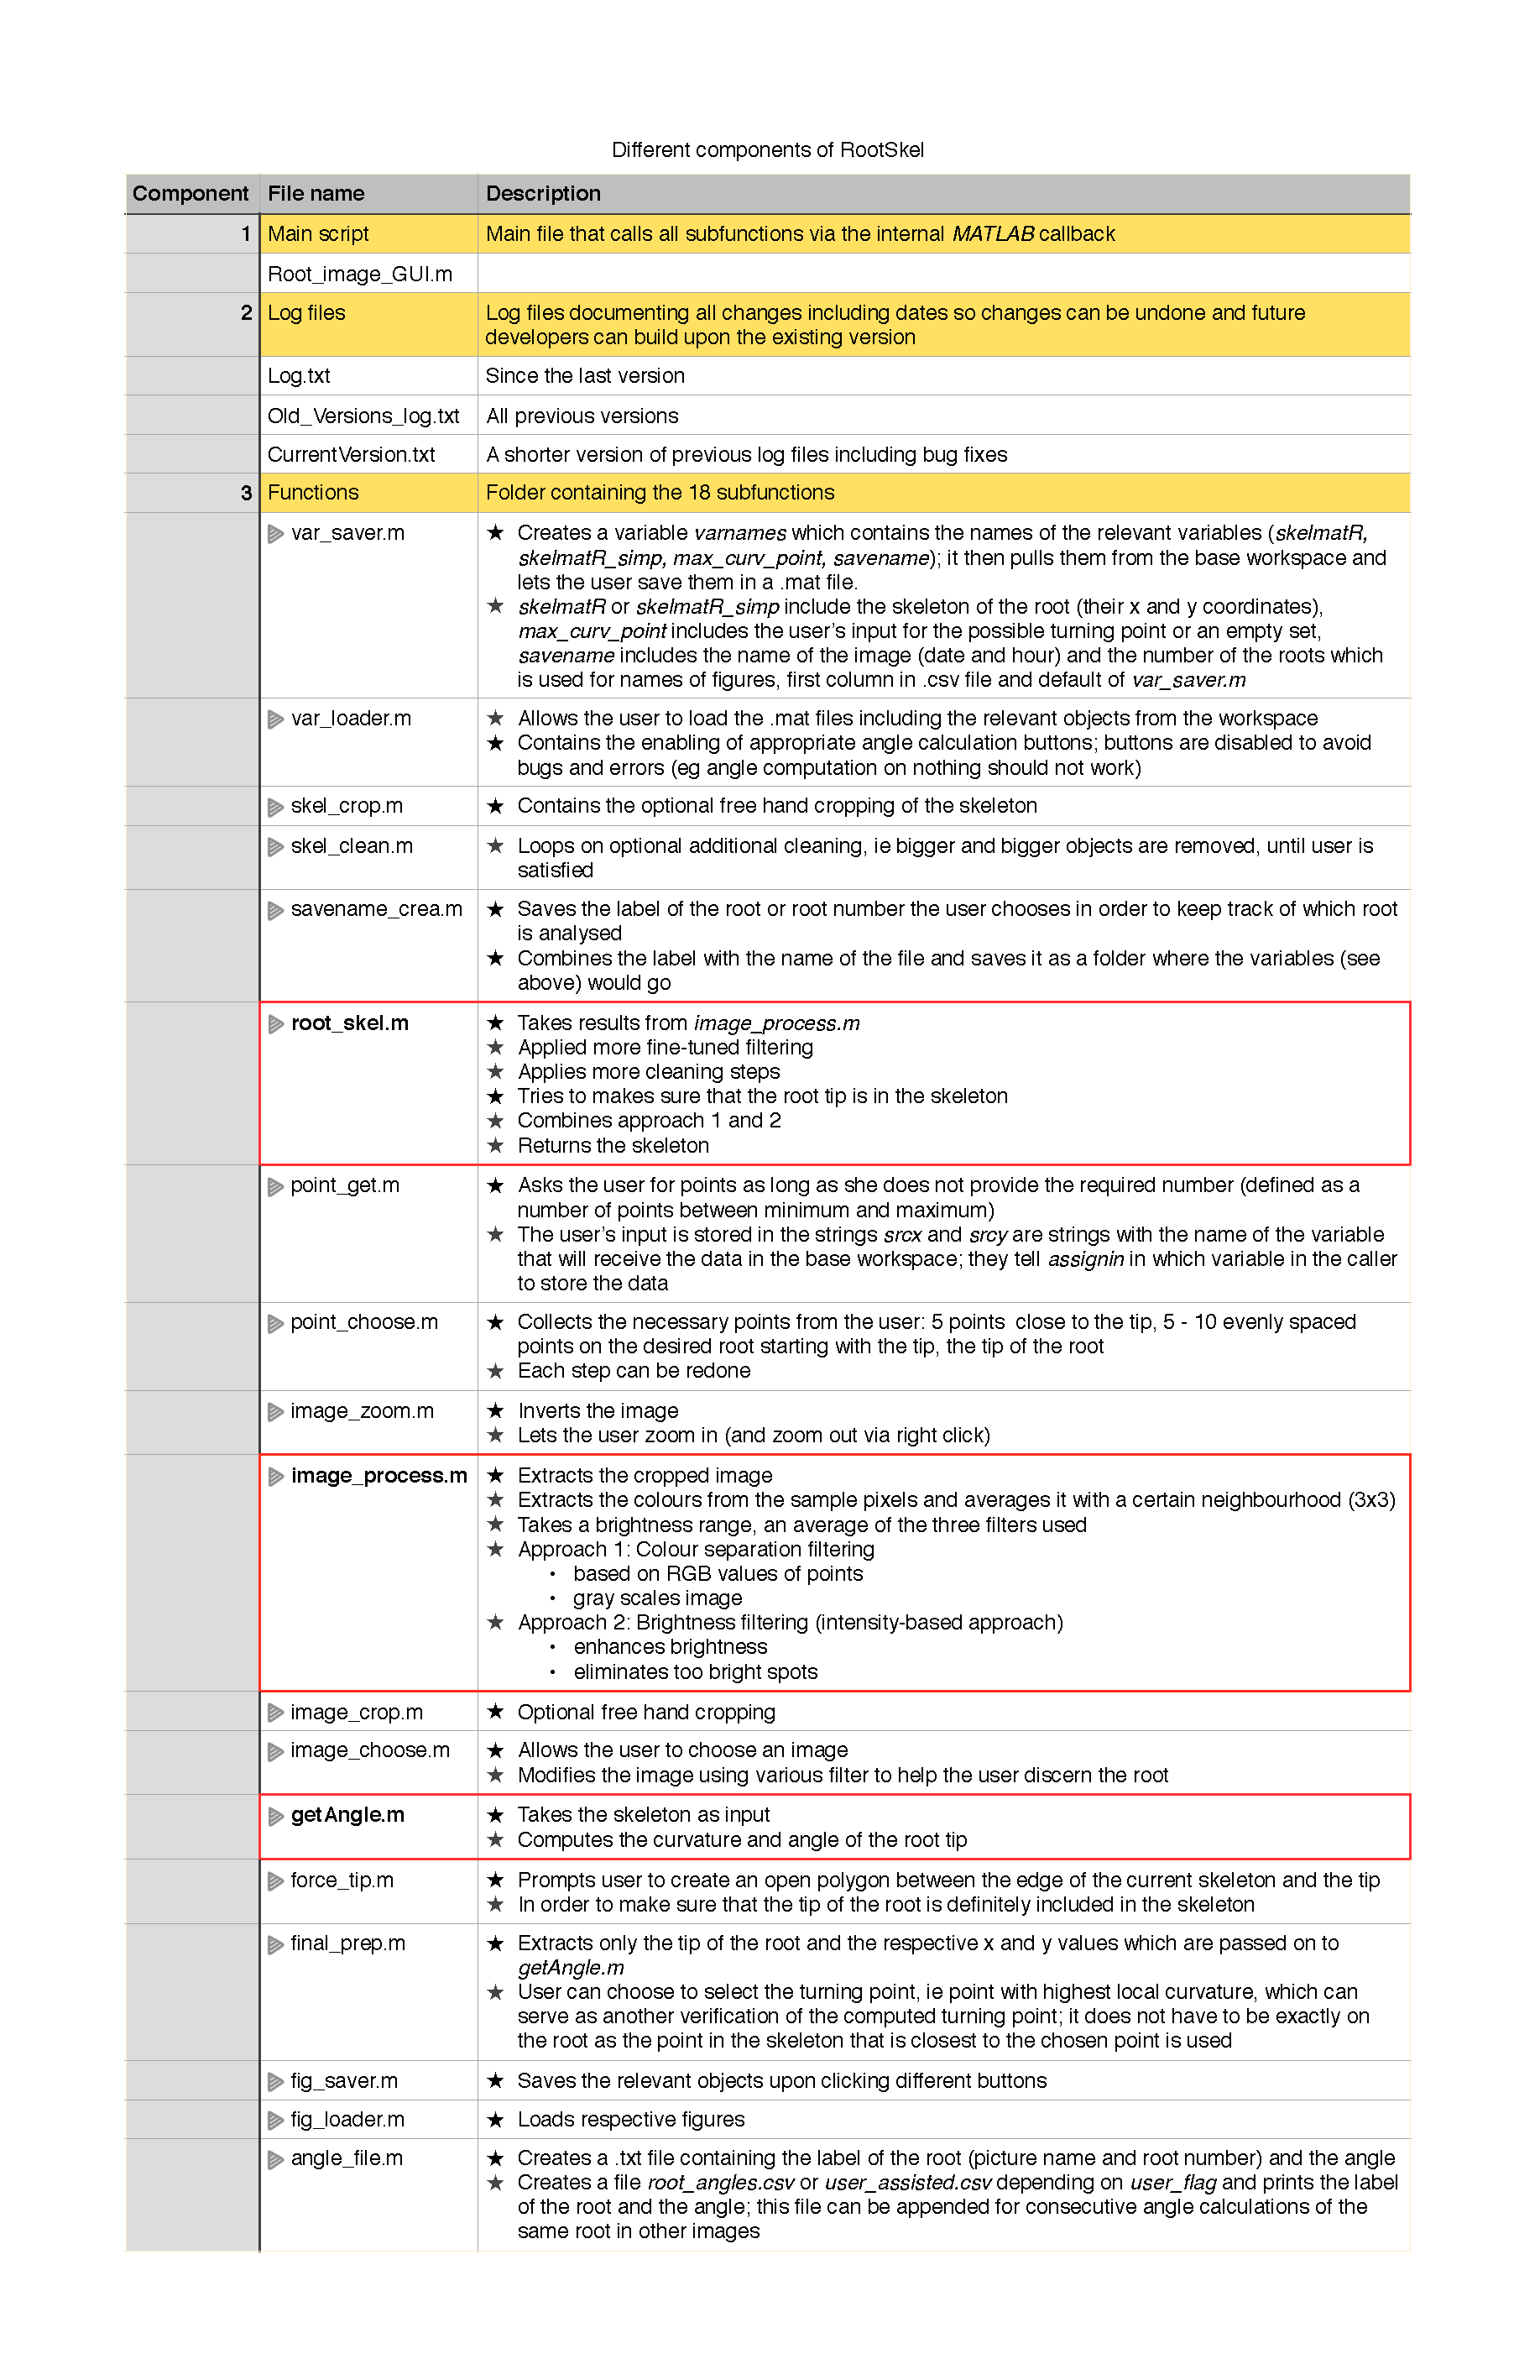
\includegraphics[width=1.\textwidth]{../Figures/components2.pdf}
	\caption{The different components and modules of \textit{RootSkel} with a description of each of them; the most important ones containing the core functionality of \textit{RootSkel} are framed in red, the high-level components are shaded in yellow.}
	\label{table:modules}
	\end{table}

%----------------------------------------------------------------------------------------
%----------------------------------------------------------------------------------------
%----------------------------------------------------------------------------------------
\chapter{Manual of \textit{RootSkel}}


%----------------------------------------------------------------------------------------
%----------------------------------------------------------------------------------------
\section{Key features} %SHOW HOW ELEABORATE TOOL IS

Figure [INSERT REFERENCE HERE: PIPELINE FROM GUI] explains the key components of this image-analysis software tool to address the problem of highly noisy electrotropism consumer camera images of Arabidopsis roots and a standardised way of computing the angle for the curved root tip. 

This tool takes the form of a MATLAB program and subprograms with a graphical user interface on top of it.

%----------------------------------------------------------------------------------------
\subsection{Handling user's mistakes}

When we take the user's input, e.g. choosing samples along the root, we correct for small mistakes by taking a neighbourhood (3\(\times\)3) average around the pixel. 
%followed by adaptive thresholding.
This means the user does not have to take special care when choosing the points as long as it is in the approximate region of the root.

%----------------------------------------------------------------------------------------
\subsection{User interaction and optional steps}
The software tool was created in ways that it is easy to interact with for a future user. 
We implemented several optional steps that only need to be performed if the user thinks they are necessary. This on the one hand saves time in the preprocessing but on the other hand also ensures that tricky roots can be tackled by various optional steps in order to extract a skeleton. 

%----------------------------------------------------------------------------------------
\subsection{Drawing the angle}
The GUI lets the user visualise the angle that is computed. This not only helps to make the tool more visual and transparent, but can also assist in debugging. 



%----------------------------------------------------------------------------------------
%----------------------------------------------------------------------------------------
%----------------------------------------------------------------------------------------
\chapter{Other programming languages}

Even though MATLAB has several advantages, it might be worth looking into alternative non-proprietary programming languages to make the tool accessible to a wider public or other options of making the tool portable, i.e. without requiring the user to have MATLAB installed.
Alternative languages one might want to consider are \textit{Python} and \textit{Julia}. Another recommended language is \textit{OpenCV} as it is very fast and well documented. Other non-open source software such as \textit{ImageJ}, a Java based image processing program, and \textit{Avizo} which is a general-purpose commercial software application for scientific and industrial data visualisation and analysis with a nice GUI, were not investigated further in this work. 


\chapter{On the data set}

The data set used can be found on [INSERT REFERENCE GITHUB HERE].

%----------------------------------------------------------------------------------------
%----------------------------------------------------------------------------------------
\section{Suggestions for future data acquisition}

We will give some suggestions on how to improve the quality of the images in the future.


%----------------------------------------------------------------------------------------
\subsection{Stable conditions in the experiment}

In general, one should ensure to keep the conditions over one experiment stable as far as possible. It should be noted that this is far harder to achieve in a dynamic system as the one to capture electrotropism compared to a gravitropism setup; the latter usually being done in a stabilising agar gel. 
This includes a constant number of tubes and roots, constant water level or surface and no external movement to the roots or the tubes to keep the noise distribution as constant as possible. Roots that are affected by change in reflections or illumination (e.g. by people walking into the room) have been proven to be very hard to handle and are often lost in the preprocessing step. 
Keeping the medium clean of dirt and bubbles as far as possible will also improve the preprocessing step. 


\subsection{No objects interfering with the object of interest}

The experimentalist should make sure that there are no objects interfering with the object of interest, be it other roots or any other similar looking objects that are hard to discern even by eye, throughout the experiment.

%llumination different — challenge to get background right
%local thresholds maybe?


%----------------------------------------------------------------------------------------
\subsection{Increase of the contrast}

It is advisable to work towards achieving a higher contrast in the images, so roots can be clearly distinguished from the background, also by eye.


%%----------------------------------------------------------------------------------------
%\subsection{More focus on images}


%----------------------------------------------------------------------------------------
\subsection{Higher resolution}


As the highly pixeled nature of the images did cause problems also in the angle computation, it is recommendable to try to increase the resolution of the images. We could also try to zoom into the roots or even one single root so our actual object(s) of interest take a bigger fraction in the images instead of spending resolution on things that are of no interest. 

It might also be the compression step after taking the images that might cause or contribute to the low resolution of the images. One could attempt to use other formats to save the images. 

As a last suggestion, different cameras could be compared to see if it does have an effect on the quality of the images. 

%Better camera, less waste of resolution
%improve spatial resolution, other format? no compression?



%%%%%%%%%%%%%%%%%%%%%%%%%%%%%%%%%%%%%%%%%%%%%
%\chapter{Data}
%
%The data was taken by a ... camera using a raspberry Pi.
%Insert details regarding data collection.
%
%\chapter{Frequently Asked Questions} % Main appendix title
%
%\label{AppendixA} % For referencing this appendix elsewhere, use \ref{AppendixA}
%
%\section{How do I change the colors of links?}
%
%The color of links can be changed to your liking using:
%
%{\small\verb!\hypersetup{urlcolor=red}!}, or
%
%{\small\verb!\hypersetup{citecolor=green}!}, or
%
%{\small\verb!\hypersetup{allcolor=blue}!}.
%
%\noindent If you want to completely hide the links, you can use:
%
%{\small\verb!\hypersetup{allcolors=.}!}, or even better: 
%
%{\small\verb!\hypersetup{hidelinks}!}.
%
%\noindent If you want to have obvious links in the PDF but not the printed text, use:
%
%{\small\verb!\hypersetup{colorlinks=false}!}.
